\chapter[%
    Linear-Response Density Cumulant Theory for Excited States:\\
	Better Algorithms, Bigger Systems
]{%
    Linear-Response Density Cumulant Theory for Excited States:\\
	Better Algorithms, Bigger Systems
}
\label{ch:davidson}


\section{Abstract}

We have recently proposed the LR-ODC-12 model for electronic excited states, a
linear response extension of density cumulant theory with linearized double
excitations and variationally optimized orbitals.
Our benchmark calculations have shown that LR-ODC-12 is consistently more
accurate than its popular equation-of-motion coupled-cluster counterpart,
EOM-CCSD\@.
Here we propose improved algorithms for solving the LR-ODC-12 equations in order
to extend its range of application to larger systems.
We use the new implementation to study the valence spectra of ethylene,
butadiene, and hexatriene.
The latter has 44 electrons and 124 spatial orbitals, a formidable challenge for
a spin-orbital code where this results in nearly 20 million unique wavefunction
parameters.
The advantages of LR-ODC-12 for these polyene systems are even more stark than
for our previous benchmarks.
Whereas EOM-CCSD overestimates the energy of the challenging
\termsymbol{2{}^1A_g} state of hexatriene and its gap with the neighboring
\termsymbol{1{}^1B_u} state by close to 1~\eV each, LR-ODC-12 matches its energy
to within 0.15~\eV and matches the energy gap to within 0.01~\eV.


\section{Introduction}

Paragraph 1:
\begin{enumerate}
    \item
        The success of ground state coupled-cluster theory comes not from CCSD
        itself, which has a relatively poor cost-accuracy ratio, but from the
        non-iterative (T) correction to CCSD, which affords truly exceptional
        accuracy relative to its cost.\cite{Stanton:1997p130}
    \item
        Coupled-cluster theory has also been extremely popular in the study of
        electronic excited states through the equation-of-motion coupled-cluster
        (EOM-CC) method,\cite{Krylov:2008p433} because it is relatively
        black-box compared to multi-reference methods like
        CASPT2\cite{Andersson:1992p1218} which require artfully chosen active
        spaces and empirical shift parameters.\cite{Zobel:2017p1482}
    \item
        Unfortunately, despite ongoing efforts to develop perturbative triples
        corrections for EOM-CCSD excitation energies, none of these attempts
        have been nearly as successful as CCSD(T).\cite{Matthews:2016p124102}
    \item
        As a result, one must resort to non-iterative triples methods like
        EOM-CC3\cite{Koch:1998p1808} or EOM-CCSDT\cite{Hirata:2000p255} to
        achieve quantitative (\(<0.1~\eV\)) accuracy, which are prohibitive even
        for modest-sized systems and basis sets.
    \item
        The LR-ODC-12 method improves on EOM-CCSD without including triples
        parameters.
\end{enumerate}


\section{Algorithms}

\begin{algorithm}
    \caption{%
        Canonical multiroot Davidson algorithm for a generalized non-symmetric
        eigenvalue problem,
        $\mathbf{L}\mathbf{v}_k=\lambda_k\mathbf{G}\mathbf{v}_k$, with periodic
        subspace collapse.
        Requires linear transformation functions and diagonal approximations
        (indicated by tildes) for \(\mathbf{L}\) and \(\mathbf{G}\)
        and solves for the lowest \(n\) eigenvalues and eigenvectors.
    }
    \label{algo:davidson}
    \begin{algorithmic}[1]
        \Procedure{Davidson}{%
            $
            \mathbf{L}(\cdot),
            \mathbf{G}(\cdot),
            \tilde{\mathbf{L}},
            \tilde{\mathbf{G}},
            \mathbf{U}^{(0)},
            n,
            d_\mathrm{max},
            i_\mathrm{max},
            r_\mathrm{tol}
            $%
        }
        \State
        Initialize the expansion space with a set of guess vectors,
        \(\mathbf{U}\leftarrow\mathbf{U}^{(0)}\).
        \For{$1\leq i\leq i_\mathrm{max}$}{}
            \State
            Construct subspace representation and solve the lowest \(n\)
            eigenvalues.
            \[
                \mathbf{L}^\mathrm{sub}
                =
                \mathbf{U}^\dagger
                \mathbf{L}(\mathbf{U})
            \]
            \[
                \mathbf{G}^\mathrm{sub}
                =
                \mathbf{U}^\dagger
                \mathbf{G}(\mathbf{U})
            \]
            \[
                \mathbf{L}^\mathrm{sub}
                \mathbf{v}_k^\mathrm{sub}
                =
                \lambda_k
                \mathbf{G}^\mathrm{sub}
                \mathbf{v}_k^\mathrm{sub}
            \]
            \State
            Calculate the eigenvector residuals over the full space.
            \[
                \mathbf{r}_k
                =
                (
                    \mathbf{L}(\mathbf{U})
                    -
                    \lambda_k
                    \mathbf{G}(\mathbf{U})
                )
                \mathbf{v}_k^\mathrm{sub}
            \]
            \If{$\max(\mathbf{r}_k) < r_\mathrm{tol}$ for all $k$}
                \State
                Set
                \(\mathbf{v}_k\leftarrow\mathbf{U}\mathbf{v}_k^\mathrm{sub}\)
                and quit the loop.  The eigenvectors are converged.
            \EndIf
            \State
            Determine new direction vectors by a quasi-Newton-Raphson step.
            \[
                \mathbf{d}_k^{(i)}
                =
                -
                (
                    \tilde{\mathbf{L}}
                    -
                    \lambda_k
                    \tilde{\mathbf{G}}
                )^{-1}
                \mathbf{r}_k
            \]
            \State
            Project out the span of \(\mathbf{U}\) and orthogonalize via
            SVD compression.
            \[
                \widehat{\mathbf{U}}^{(i)}
                =
                (\mathbf{1} - \mathbf{U}^\dagger \mathbf{U})
                \mathbf{D}^{(i)}
            \]
            \[
                \widehat{\mathbf{U}}^{(i)}
                \approx
                \mathbf{U}^{(i)}
                \mathbf{\Sigma}^{(i)}
                \mathbf{W}^{(i)\dagger}
            \]
            \If{%
                $
                \mathrm{rank}(\mathbf{U})
                +
                \mathrm{rank}(\mathbf{U}^{(i)})
                <
                d_\mathrm{max}
                $%
            }
                \State
                Extend the expansion space,
                \(
                    \mathbf{U}
                    \leftarrow
                    (\mathbf{U}\ \mathbf{U}^{(i)})
                \)
            \Else
                \State
                Collapse the expansion space,
                \(
                    \mathbf{U}
                    \leftarrow
                    (
                        \mathbf{U}
                        \mathbf{v}_1^\mathrm{sub}\ 
                        \cdots\ 
                        \mathbf{U}
                        \mathbf{v}_n^\mathrm{sub}
                    )
                \).
            \EndIf
        \EndFor
        \State
        {\bfseries return}
        \(
            \lambda_k,
            \mathbf{v}_k
        \)
        \EndProcedure
    \end{algorithmic}
\end{algorithm}

The LR-ODC-12 eigenvalue equation has a two-by-two block structure which
describes the independent variation of the state parameters and their complex
conjugates.
\begin{equation}
    \label{eq:linear-response-eigenvalue-equation}
    \mathbf{E}(\mathbf{z}_k)
    =
    \omega_k
    \mathbf{M}(\mathbf{z}_k)
    ,
    \quad
    \mathbf{E}
    =
    \begin{pmatrix}
        \mathbf{A} & \mathbf{B} \\
        \mathbf{B}^* & \mathbf{A}^*
    \end{pmatrix}
    ,
    \quad
    \mathbf{M}
    =
    \begin{pmatrix}
        \mathbf{S} & \mathbf{0} \\
        \mathbf{0} & -\mathbf{S}^*
    \end{pmatrix}
    ,
    \quad
    \mathbf{z}_k
    =
    \begin{pmatrix}
        \mathbf{x}_k \\
        \mathbf{y}_k
    \end{pmatrix}
\end{equation}
This block symmetry leads to a paired system of eigenvalues,
\(
    \omega_{\pm k}
    =
    \pm\omega_k
\).
The submatrices in \cref{eq:linear-response-eigenvalue-equation} are further
blocked according to whether they describe variations with respect to one-body
(\(\mathbf{t}_1\)) or two-body (\(\mathbf{t}_2\)) parameters.
\begin{equation}
    \label{eq:conjugate-blocks}
    \mathbf{A}
    =
    \begin{pmatrix}
        \mathbf{A}_{11} & \mathbf{A}_{12} \\
        \mathbf{A}_{21} & \mathbf{A}_{22} \\
    \end{pmatrix}
    \quad
    \mathbf{B}
    =
    \begin{pmatrix}
        \mathbf{B}_{11} & \mathbf{B}_{12} \\
        \mathbf{B}_{21} & \mathbf{B}_{22} \\
    \end{pmatrix}
    \quad
    \mathbf{S}
    =
    \begin{pmatrix}
        \mathbf{S}_{11} & \mathbf{0} \\
        \mathbf{0} & \mathbf{1}_2 \\
    \end{pmatrix}
    \quad
    \mathbf{x}_k
    =
    \begin{pmatrix}
        \mathbf{x}_{k,1} \\
        \mathbf{x}_{k,2}
    \end{pmatrix}
\end{equation}
The dimensions of the diagonal two-body blocks (\(\mathbf{A}_{22}\) and
\(\mathbf{B}_{22}\) and \(\mathbf{1}_s\)) in these matrices scale as
\((\mathrm{o}^2\mathrm{v}^2)^2\) with the number of occupied (\(\mathrm{o}\))
and virtual (\(\mathrm{v}\)) orbitals, rapidly overwhelming the storage space on
a given computer as the number of electrons and basis functions increases.
This problem can be circumvented by using so-called ``direct'' matrix
algorithms, which avoid the explicit representation of a matrix as an array of
coefficients \(\mathbf{L}=[L_{\mu\nu}]\) by instead defining a function
\(\mathbf{L}(\mathbf{U})\) which returns the output of the linear transformation
on an arbitrary set of vectors \(\mathbf{U}=(\mathbf{u}_1\ \cdots\
\mathbf{u}_m)\).
The standard direct algorithm for extremal eigenvalues of large,
diagonally-dominant matrices is the Davidson
algorithm,\cite{Davidson:1975p87,Liu:1978p49} which solves the eigenvalue
problem by progressively growing an expansion space for the \(n\) lowest (or
highest) generalized eigenvectors.
The procedure is described in \Cref{algo:davidson}.

The full set of linear transformation formulas for the LR-ODC-12 Hessian and
metric blocks is given in the appendix
(\cref{sec:linear-transformation-formulas}), but let us consider the diagonal
two-body Hessian as an example.
The image of an arbitrary two-body vector
\(
    \mathbf{u}_{\mu,2}
    =
    [u_{\mu,ab}^{ij}]
\)
under this transformation is given by
\begin{equation}
    \label{eq:two-body-hessian-function-in-text}
    \begin{array}{r@{\,}l}
        (\mathbf{A}_{22}(\mathbf{u}_{\mu,2}))_{ijab}
        =
        &
        -
        P_{(a/b)}
        \mathcal{F}_a^c
        u_{\mu,cb}^{ij}
        -
        P^{(i/j)}
        \mathcal{F}_k^i
        u_{\mu,ab}^{kj}
        +
        \tfrac{1}{2}
        \overline{g}_{ab}^{cd}
        u_{\mu,cd}^{ij}
        +
        \tfrac{1}{2}
        \overline{g}_{kl}^{ij}
        u_{\mu,ab}^{kl}
        \\[5pt]
        &
        -
        P_{(a/b)}^{(i/j)}
        \overline{g}_{la}^{jc}
        u_{\mu,cb}^{il}
        +
        \tfrac{1}{2}
        P_{(a/b)}
        \mathcal{G}_{af}^{ec}
        t_{eb}^{ij}
        t_{kl}^{fd*}
        u_{\mu,cd}^{kl}
        +
        \tfrac{1}{2}
        P_{(a/b)}
        \mathcal{G}_{ka}^{me}
        t_{eb}^{ij}
        t_{ml}^{cd*}
        u_{\mu,cd}^{kl}
        \\[5pt]
        &
        +
        \tfrac{1}{2}
        P^{(i/j)}
        \mathcal{G}_{me}^{ic}
        t_{ab}^{mj}
        t_{kl}^{ed*}
        u_{\mu,cd}^{kl}
        +
        \tfrac{1}{2}
        P^{(i/j)}
        \mathcal{G}_{mk}^{in}
        t_{ab}^{mj}
        t_{nl}^{cd*}
        u_{\mu,cd}^{kl}
    \end{array}
\end{equation}
where the \(i,j,k,l,\ldots\) run over occupied spin-orbitals, \(a,b,c,d,\ldots\)
run over virtual (un-occupied) spin-orbitals, and summation over repeated
indices is implied.
The important thing to note is that we need only two \(\mathrm{v}^4\)-sized
intermediates (\(\overline{g}_{ab}^{cd}\) and \(\mathcal{G}_{ab}^{cd}\)) to
define our linear transformations, and that the image of the two-body Hessian
only has \(\mathcal{O}(d_\mu\mathrm{o}^2\mathrm{v}^2)\) elements where \(d_\mu\)
is the dimension of the \(\mu\) index.
In general the Davidson algorithm requires no more than 10-20 subspace vectors
per root, sometimes as few as 2 or 3, so that even for small systems it is easy
to satisfy \( d_\mu \ll \mathrm{o}^2\mathrm{v}^2 \), resulting in substantial
memory savings.
\Cref{eq:two-body-hessian-function-in-text} also includes the timing bottleneck
for the LR-ODC-12, the contraction of the \(\mathrm{v}^4\) integrals with the
expansion vector, \(\mathrm{g}_{ab}^{cd}u_{\mu,cd}^{ij}\), which scales as
\(\mathcal{O}(d_\mu\mathrm{o}^2\mathrm{v}^4)\) in the number of floating point
operations.
This term is the rate limiting step in EOM-CCSD as well.

A direct application of \cref{algo:davidson} to
\cref{eq:linear-response-eigenvalue-equation} is complicated by the fact that
the desired (small, positive) eigenvalues are in the middle of the spectrum,
rather than at the extremes.
We make use of two strategies.

\begin{figure}[h!]
    \centering
    \caption{%
        \label{fig:davidson}
        A schematic illustrating the sequence of reduced representations of
        \(\mathbf{E}\) in a blocked Davidson algorithm.
        The colored entries must be explicitly computed, whereas the gray
        entries are determined by Hermitian symmetry.
    }
    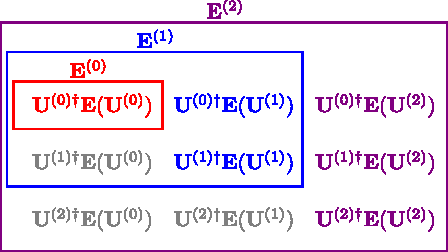
\includegraphics[width=8.5cm]{figures/davidson.pdf}
\end{figure}


\paragraph{Strategy 1}
One approach is to invert the eigenvalue equation, solving for the {\itshape
largest} positive inverse eigenvalues, which is easily done by selecting the
highest rather than the lowest roots at each step in \cref{algo:davidson}.
\begin{equation}
    \mathbf{M}(\mathbf{z}_k)
    =
    \omega_k^{-1}
    \mathbf{E}(\mathbf{z}_k)
\end{equation}
This has the added advantage that the energy Hessian \(\mathbf{E}\) is generally
positive definite, which allows us to treat the subspace diagonalizations as
standard Hermitian eigenvalue equation with real eigenvalues and orthonormal
eigenvectors.
A simple, effective choice of guess vectors in this approach is to determine the
lowest eigenvectors of the following diagonal approximation to
\cref{eq:two-body-hessian-function-in-text}
\begin{equation}
    (\tilde{\mathbf{A}}_{22}(\mathbf{u}_{\mu}))_{ijab}
    \equiv
    -
    (
        \mathcal{F}_i^i
        +
        \mathcal{F}_j^j
        +
        \mathcal{F}_a^a
        +
        \mathcal{F}_b^b
    )
    u_{\mu,ab}^{ij}
\end{equation}
which are simply the standard unit vectors associated with the smallest diagonal
entries.
The virtual coefficients \(\mathcal{F}_a^a,\mathcal{F}_b^b\) in this equation
are generally negative, so this has the form of an orbital energy difference
like we see in Hartree-Fock theory.
For larger systems, we manage the memory requirements of the method by keeping
successive groups of expansion vectors and images,
\(
    \mathbf{U}^{(i)},
    \mathbf{E}(\mathbf{U}^{(i)}),
    \mathbf{M}(\mathbf{U}^{(i)})
\),
on disk and reading them in as needed.
These can be further subdivided into even smaller blocks if needed.
\Cref{fig:davidson} illustrates which entries in the subspace representation
need to be explicitly computed as we add vectors to the expansion space.


\paragraph{Strategy 2}
Assuming real matrices, we can add and subtract the block rows of
\cref{eq:linear-response-eigenvalue-equation} to arrive at the following pair of
equations.
\begin{equation}
    (\mathbf{A} \pm \mathbf{B})
    (\mathbf{x}_k  \pm \mathbf{y}_k)
    =
    \omega_k
    \mathbf{S}
    (\mathbf{x}_k \mp \mathbf{y}_k)
\end{equation}
Substituting one into the other leads to a non-symmetric eigenvalue equation for
the squares of the excitation energies.
\begin{equation}
    \widehat{\mathbf{E}}
    (\mathbf{x}_k - \mathbf{y}_k)
    =
    \omega_k^2
    (\mathbf{x}_k - \mathbf{y}_k)
    ,
    \quad
    \widehat{\mathbf{E}}
    \equiv
    \mathbf{S}^{-1}
    (\mathbf{A} + \mathbf{B})
    \mathbf{S}^{-1}
    (\mathbf{A} - \mathbf{B})
\end{equation}
By halving the dimension of the problem and eliminating the metric, this reduces
the memory requirements by a factor of three, provided we do not need to recover
the full eigenvector \(\mathbf{z}_k\) to compute transition properties.
From \cref{eq:conjugate-blocks} we can see that computing the inverse of
\(\mathbf{S}\) requires us to invert the orbital block of the metric.


\begin{equation}
    \mathbf{E}(\mathbf{Z})
    =
    \mathbf{M}(\mathbf{Z})
    \boldsymbol{\Omega}
\end{equation}
Need not be square

\begin{equation}
    \mathbf{Z}
    =
    \begin{pmatrix}
        \mathbf{X}_1 \\
        \mathbf{X}_2 \\
        \mathbf{Y}_1 \\
        \mathbf{Y}_2
    \end{pmatrix}
\end{equation}

\begin{equation}
    \mathbf{E}(\mathbf{Z})
    =
    \begin{pmatrix}
        \mathbf{A}_{11}(\mathbf{X}_1) +
        \mathbf{A}_{12}(\mathbf{X}_2) +
        \mathbf{B}_{11}(\mathbf{Y}_1) +
        \mathbf{B}_{12}(\mathbf{Y}_2) \\
        \mathbf{A}_{21}(\mathbf{X}_1) +
        \mathbf{A}_{22}(\mathbf{X}_2) +
        \mathbf{B}_{21}(\mathbf{Y}_1) +
        \mathbf{B}_{22}(\mathbf{Y}_2) \\
        \mathbf{B}^*_{11}(\mathbf{X}_1) +
        \mathbf{B}^*_{12}(\mathbf{X}_2) +
        \mathbf{A}^*_{11}(\mathbf{Y}_1) +
        \mathbf{A}^*_{12}(\mathbf{Y}_2) \\
        \mathbf{B}^*_{21}(\mathbf{X}_1) +
        \mathbf{B}^*_{22}(\mathbf{X}_2) +
        \mathbf{A}^*_{21}(\mathbf{Y}_1) +
        \mathbf{A}^*_{22}(\mathbf{Y}_2) \\
    \end{pmatrix}
\end{equation}


    We have implemented the LR-ODC-12 method using a multi-root Davidson algorithm,
    which solves the linear-response generalized eigenvalue problem by progressively
    growing an expansion space for the \(n_\mathrm{root}\) lowest generalized
    eigenvectors of \(\mathbf{E}\) and \(\mathbf{M}\).
    The general procedure looks as follows:
    \begin{enumerate}
        \item
            \label{item:davidson-initialization}
            Initialize the expansion space with a set of \(n_\mathrm{guess}\geq
            n_\mathrm{root}\) orthonormal vectors.
            \[
                \mathbf{R}^{(0)}
                =
                (
                    \mathbf{u}_1^{(0)}
                    \cdots
                    \mathbf{u}_{n_\mathrm{guess}}^{(0)}
                )
            \]
        \item
            \label{item:davidson-step-one}
            Express the energy-Hessian and metric matrices in the reduced expansion
            space.
            \[
                \mathbf{E}^{(i)}
                =
                \mathbf{R}^{(i)\dagger}
                \mathbf{E}(\mathbf{R}^{(i)})
            \]
            \[
                \mathbf{M}^{(i)}
                =
                \mathbf{R}^{(i)\dagger}
                \mathbf{M}(\mathbf{R}^{(i)})
            \]
        \item
            Solve for the \(n_\mathrm{root}\) highest eigenvectors of the
            inverse eigenvalue equation.
            \[
                \mathbf{M}^{(i)}
                \mathbf{z}_k^{(i)}
                =
                \mathbf{E}^{(i)}
                \mathbf{z}_k^{(i)}/
                \omega_k^{(i)}
            \]
        \item
            Determine the residual for each root.
            \[
                \mathbf{d}_k^{(i)}
                =
                \mathbf{M}(\mathbf{z}_k^{(i)})
                -
                \mathbf{E}(\mathbf{z}_k^{(i)})/
                \omega_k^{(i)}
            \]
            If the residual elements are sufficiently small we consider the
            eigenvectors converged and exit the loop.
        \item
            \label{item:davidson-step-three}
            Form new direction vectors by preconditioning the residuals.
            \[
                \mathbf{g}_k^{(i+1)}
                =
                -
                (
                    \tilde{\mathbf{M}}
                    -
                    \tilde{\mathbf{E}}/
                    \omega_k^{(i)}
                )^{-1}
                \mathbf{d}_k
            \]
            The tildes in this equation denote diagonal approximations to these
            matrices.
        \item
            Project out the span of the current expansion space from the new
            direction vectors.
            \[
                \mathbf{J}^{(i+1)}
                =
                (\mathbf{1} - \mathbf{R}^{(i)}\mathbf{R}^{(i)\dagger})
                (\mathbf{g}_1^{(i+1)}\cdots \mathbf{g}_{n_\mathrm{root}}^{(i+1)})
            \]
        \item
            Determine an orthonormal basis for the new direction vectors using a
            compressed singular value decomposition, and add these new vectors to
            the expansion space.
            \[
                \mathbf{J}^{(i+1)}
                \approx
                \mathbf{U}^{(i+1)}
                \boldsymbol\Sigma^{(i+1)}
                \mathbf{V}^{(i+1)\dagger}
            \]
            \[
                \mathbf{R}^{(i+1)}
                \leftarrow
                (\mathbf{R}^{(i)}\ \mathbf{U}^{(i+1)})
            \]
        \item
            Increment \(i\) and return to step~\ref{item:davidson-step-one}.
    \end{enumerate}
    A key feature of this algorithm is that we never need to explicilty construct
    the energy-Hessian and metric matrices in memory, only their images over the
    expansion space.

    For the diagonal approximations in step~\ref{item:davidson-step-three} we use
    the following.
    \[
        \tilde{\mathbf{S}}_{11}
        \equiv
        \mathbf{1}_1
    \]
    \[
        (\tilde{\mathbf{A}}_{11})_{ia,ia}
        \equiv
        -
        f_i^i
        +
        f_a^a
    \]
    \[
        (\tilde{\mathbf{A}}_{22})_{ijab,ijab}
        \equiv
        -
        \mathcal{F}_i^i
        -
        \mathcal{F}_j^j
    -
    \mathcal{F}_a^a
    -
    \mathcal{F}_b^b
\]
These can also be used to construct the initial expansion space in
step~\ref{item:davidson-initialization}, namely by including unit vectors for
the \(n_\mathrm{guess}\) smallest positive entries in \(\tilde{\mathbf{E}}\).


\section{Computational Details}

For alkenes (\cref{sec:alkenes}), the ANO-L-pVXZ (X = D, T) basis
sets\cite{Widmark:1990p291} were used as in Ref.~\citenum{Daday:2012p4441}.
For alkenes in \cref{sec:alkenes}, the frozen-core MP2/cc-pVQZ geometries were
used as in Refs.~\citenum{Daday:2012p4441} and \citenum{Zimmerman:2017p4712}.


\section{Results and Discussion}
\label{sec:alkenes}

\begin{table*}[h!]
    \centering
    \caption{%
        \label{tab:alkenes}
        Vertical excitation energies computed using LR-OLCCD, LR-ODC-12, and
        EOM-CCSD for the low-lying electronic states of ethylene (\ce{C2H4}),
        butadiene (\ce{C4H6}), and hexatriene (\ce{C6H8}).
        Computations employed the ANO-L-pVDZ (for \ce{C4H6} and \ce{C6H8}) and
        ANO-L-pVTZ (for \ce{C2H4}) basis sets and the MP2/cc-pVQZ optimized
        geometries.
        For LR-OLCCD and LR-ODC-12, oscillator strengths of the allowed
        transitions are given in parentheses.
        All electrons were correlated in all computations.
    }
    \begin{threeparttable}
        \begin{tabular}{clccccc}
            \hline
            \hline
            && EOM-CCSD & LR-OLCCD & LR-ODC-12 & SHCI\tnote{a} \\
            \hline
            \ce{C2H4}
            & \(1{}^3\mathrm{B_{1u}}\) &
            4.46 & 4.66         & 4.52         & 4.59  \\ 
            & \(1{}^1\mathrm{B_{1u}}\) &
            8.14 & 8.20 (1.8) & 8.14 (1.9) & 8.05 \\
            \hline                           
            \ce{C4H6}                        
            & \(1{}^3\mathrm{B_{u}}\)  &
            3.20 & 3.58 & 3.43 & 3.37 \\
            & \(1{}^1\mathrm{B_{u}}\)  &
            6.53 & 6.76 (4.2) & 6.67 (4.4) & 6.45 \\
            & \(2{}^1\mathrm{A_{g}}\)  &
            7.28 & 7.14 & 6.81 & 6.58 \\
            \hline                           
            \ce{C6H8}                        
            & \(1{}^3\mathrm{B_{u}}\)  &
            2.64 & 3.01 & 2.83 & 2.77 \\
            & \(1{}^1\mathrm{B_{u}}\)  &
            5.60 & 5.89 (6.5)  & 5.74 (8.1)   & 5.59 \\
            & \(2{}^1\mathrm{A_{g}}\)  &
            6.55 & 4.21 & 5.73 & 5.58 \\
            \hline
            \hline
        \end{tabular}
        \begin{tablenotes}
            \item[a]
                Also shown are the excitation energies from the semistochastic
                heat-bath CI (SHCI) method, extrapolated to full CI
                limit.\cite{Chien:2018p2714}
                The $1s$ orbitals of carbon atoms were not included in the SHCI
                correlation treatment.
                The SHCI computations used the same basis sets and optimized
                geometries as those used for LR-OLCCD, LR-ODC-12, and EOM-CCSD.
        \end{tablenotes}    
    \end{threeparttable}
\end{table*}


We apply the LR-ODC-12 method to challenging excited states of ethylene
(\ce{C2H4}), butadiene (\ce{C4H6}), and hexatriene (\ce{C6H8}).  A reliable
description of these electronic states requires accurate treatment of electron
correlation.\cite{%
    Tavan:1986p6602, Tavan:1987p4337, Nakayama:1998p157,
    Davidson:1996p6161, Watts:1998p6979, Muller:1999p7176, Li:1999p177,
    Starcke:2006p39, Kurashige:2004p425, Ghosh:2008p144117, Sokolov:2017p244102,
    Schreiber:2008p134110, Zgid:2009p194107, Angeli:2010p2436, Daday:2012p4441,
    Watson:2012p4013, Zimmerman:2017p4712%
}
All three molecules feature a dipole-allowed $1{}^1\mathrm{B_{u}}$ (or
$1{}^1\mathrm{B_{1u}}$) state that is well described by a $\pi-\pi^*$
excitation, but requires a very accurate description of dynamic correlation
between the $\sigma$ and $\pi$ electrons.
In butadiene and hexatriene, the $1{}^1\mathrm{B_{u}}$ state is near-degenerate
with a dipole-forbidden $2{}^1\mathrm{A_{g}}$ state that has a substantial
double-excitation character, requiring the description of static correlation in
the $\pi$ and $\pi^*$
orbitals.\cite{Kurashige:2004p425,Ghosh:2008p144117,Sokolov:2017p244102}
For this reason, the relative energies and ordering of the $1{}^1\mathrm{B_{u}}$
and $2{}^1\mathrm{A_{g}}$ states are very sensitive to various levels of theory.
For example, single-reference methods truncated to single and double excitations
are usually more accurate in describing the $1{}^1\mathrm{B_{u}}$ state than the
$2{}^1\mathrm{A_{g}}$ state, while multi-reference methods are more reliable for
the $2{}^1\mathrm{A_{g}}$ state, missing important dynamic correlation for the
$1{}^1\mathrm{B_{u}}$ state.
Very recently, Chien et al.\cite{Chien:2018p2714} reported accurate vertical
excitation energies for the low-lying states of ethylene, butadiene, and
hexatriene computed using semistochastic heat-bath configuration interaction
(SHCI) extrapolated to the full CI limit.
In this section, we will use the SHCI results to benchmark the accuracy of the
LR-ODC-12 method.

\Cref{tab:alkenes} reports the vertical excitation energies of ethylene,
butadiene, and hexatriene computed using the EOM-CCSD, LR-OLCCD, and LR-ODC-12
methods, along with the SHCI results from Ref.\@ \citenum{Chien:2018p2714}.
All methods employed the same optimized geometries and basis sets (see
\cref{tab:alkenes} for details).
We refer to the $\mathrm{B_{1u}}$ states of \ce{C2H4} as $\mathrm{B_{u}}$ for
brevity.
All excitation energies decrease as the number of double bonds increases.
For butadiene and hexatriene, the ($1{}^1\mathrm{B_{u}}$; $2{}^1\mathrm{A_{g}}$)
excitation energies computed using the SHCI method are (6.45; 6.58) and (5.59;
5.58) eV, respectively, indicating that the two states are nearly degenerate for
the longer polyene.
This feature is not reproduced by the EOM-CCSD method, which predicts the
$1{}^1\mathrm{B_{u}}$ state energies in close agreement with SHCI, but
significantly overestimates the energies for the doubly-excited
$2{}^1\mathrm{A_{g}}$ state.
As a result, the EOM-CCSD method overestimates the energy spacing between the
$1{}^1\mathrm{B_{u}}$ and $2{}^1\mathrm{A_{g}}$ states by $\sim$ 0.6 eV and 1.0
eV for butadiene and hexatriene, respectively. 

On the contrary, the LR-ODC-12 method correctly describes the relative energies
and ordering of the $1{}^1\mathrm{B_{u}}$ and $2{}^1\mathrm{A_{g}}$ states,
predicting their energy spacing to be 0.14 and 0.01 eV for butadiene and
hexatriene, respectively, in an excellent agreement with the SHCI results (0.13
and 0.01 eV).
For the singlet excited states, the LR-ODC-12 method consistently overestimates
the SHCI excitation energies by $\sim$ 0.1 -- 0.2 eV.
For the $1{}^3\mathrm{B_{u}}$ state, the LR-ODC-12 errors are smaller in
magnitude ($\sim$ 0.06 eV).
Importantly, these results suggest that the LR-ODC-12 method provides a balanced
description of the excited states with different electronic structure effects,
as illustrated by its consistent performance for the $1{}^3\mathrm{B_{u}}$,
$1{}^1\mathrm{B_{u}}$, and $2{}^1\mathrm{A_{g}}$ states in ethylene, butadiene,
and hexatriene.

Comparing the LR-ODC-12 and the LR-OLCCD results suggests that including the
non-linear terms in the description of electron correlation significantly
improves the agreement with the reference SHCI data.
In particular, for the $1{}^3\mathrm{B_{u}}$ and $1{}^1\mathrm{B_{u}}$ states,
the LR-OLCCD errors are larger than the LR-ODC-12 errors by $\sim$ 0.15 eV.
For the doubly-excited $2{}^1\mathrm{A_{g}}$ state, LR-OLCCD shows very large
errors of 0.56 and $-$1.37 eV for butadiene and hexatriene, respectively.
These results indicate that the non-linear terms included in LR-ODC-12 are very
important for the description of excited states with double-excitation
character.



\begin{subappendices}
    \section{LR-ODC-12 Linear Transformation Formulas}
    \label{sec:linear-transformation-formulas}

    \begin{equation}
        \begin{array}{r@{\,}l}
            (\mathbf{A}_{11}(\mathbf{u}_{\mu,1}))_{ia}
            =
            &
            h_j^i
            \gamma_a^b
            u_{\mu,b}^j
            +
            h_a^b
            \gamma_j^i
            u_{\mu,b}^j
            -
            (\bar{\mathbf{F}})_j^i
            u_{\mu,a}^j
            -
            (\bar{\mathbf{F}})_a^b
            u_{\mu,b}^i
            +
            \overline{g}_{nj}^{mi}
            \gamma_{ma}^{nb}
            u_{\mu,b}^j
            \\[5pt]
            &
            +
            \overline{g}_{ma}^{nb}
            \gamma_{nj}^{mi}
            u_{\mu,b}^j
            +
            \overline{g}_{jf}^{ie}
            \gamma_{ae}^{bf}
            u_{\mu,b}^j
            +
            \overline{g}_{ae}^{bf}
            \gamma_{jf}^{ie}
            u_{\mu,b}^j
            +
            \overline{g}_{me}^{ib}
            \gamma_{ja}^{me}
            u_{\mu,b}^j
            \\[5pt]
            &
            +
            \overline{g}_{ja}^{me}
            \gamma_{me}^{ib}
            u_{\mu,b}^j
        \end{array}
    \end{equation}

    \begin{equation}
        \begin{array}{r@{\,}l}
            (\mathbf{B}_{11}(\mathbf{u}_{\mu,1}))_{ia}
            =
            &
            \overline{g}_{be}^{im}
            \gamma_{ma}^{je}
            u_{\mu,j}^b
            +
            \overline{g}_{ma}^{je}
            \gamma_{be}^{im}
            u_{\mu,j}^b
            +
            \overline{g}_{mb}^{ie}
            \gamma_{ae}^{jm}
            u_{\mu,j}^b
            +
            \overline{g}_{ae}^{jm}
            \gamma_{mb}^{ie}
            u_{\mu,j}^b
            \\[5pt]
            &
            +
            \tfrac{1}{2}
            \overline{g}_{mn}^{ij}
            \gamma_{ab}^{mn}
            u_{\mu,j}^b
            +
            \tfrac{1}{2}
            \overline{g}_{ab}^{mn}
            \gamma_{mn}^{ij}
            u_{\mu,j}^b
            +
            \tfrac{1}{2}
            \overline{g}_{ef}^{ij}
            \gamma_{ab}^{ef}
            u_{\mu,j}^b
            +
            \tfrac{1}{2}
            \overline{g}_{ab}^{ef}
            \gamma_{ef}^{ij}
            u_{\mu,j}^b
        \end{array}
    \end{equation}

    \begin{equation}
        \begin{array}{r@{\,}l}
            (\mathbf{A}_{22}(\mathbf{u}_{\mu,2}))_{ijab}
            =
            &
            -
            P_{(a/b)}
            \mathcal{F}_a^c
            u_{\mu,cb}^{ij}
            -
            P^{(i/j)}
            \mathcal{F}_k^i
            u_{\mu,ab}^{kj}
            +
            \tfrac{1}{2}
            \overline{g}_{ab}^{cd}
            u_{\mu,cd}^{ij}
            +
            \tfrac{1}{2}
            \overline{g}_{kl}^{ij}
            u_{\mu,ab}^{kl}
            \\[5pt]
            &
            -
            P_{(a/b)}^{(i/j)}
            \overline{g}_{la}^{jc}
            u_{\mu,cb}^{il}
            +
            \tfrac{1}{2}
            P_{(a/b)}
            \mathcal{G}_{af}^{ec}
            t_{eb}^{ij}
            t_{kl}^{fd*}
            u_{\mu,cd}^{kl}
            +
            \tfrac{1}{2}
            P_{(a/b)}
            \mathcal{G}_{ka}^{me}
            t_{eb}^{ij}
            t_{ml}^{cd*}
            u_{\mu,cd}^{kl}
            \\[5pt]
            &
            +
            \tfrac{1}{2}
            P^{(i/j)}
            \mathcal{G}_{me}^{ic}
            t_{ab}^{mj}
            t_{kl}^{ed*}
            u_{\mu,cd}^{kl}
            +
            \tfrac{1}{2}
            P^{(i/j)}
            \mathcal{G}_{mk}^{in}
            t_{ab}^{mj}
            t_{nl}^{cd*}
            u_{\mu,cd}^{kl}
        \end{array}
    \end{equation}

    \begin{equation}
        \begin{array}{r@{\,}l}
            (\mathbf{B}_{22}(\mathbf{u}_{\mu,2}))_{ijab}
            =
            &
            \tfrac{1}{2}
            P_{(a/b)}
            \mathcal{G}_{ac}^{ef}
            t_{eb}^{ij}
            t_{fd}^{kl}
            u_{\mu,kl}^{cd}
            +
            \tfrac{1}{2}
            P_{(a/b)}
            \mathcal{G}_{na}^{ke}
            t_{eb}^{ij}
            t_{cd}^{nl}
            u_{\mu,kl}^{cd}
            \\[5pt]
            &
            +
            \tfrac{1}{2}
            P^{(i/j)}
            \mathcal{G}_{mc}^{if}
            t_{ab}^{mj}
            t_{fd}^{kl}
            u_{\mu,kl}^{cd}
            +
            \tfrac{1}{2}
            P^{(i/j)}
            \mathcal{G}_{mn}^{ik}
            t_{ab}^{mj}
            t_{cd}^{nl}
            u_{\mu,kl}^{cd}
        \end{array}
    \end{equation}

    \begin{equation}
        \begin{array}{r@{\,}l}
            (\mathbf{A}_{12}(\mathbf{u}_{\mu,2}))_{ia}
            =
            &
            \tfrac{1}{2}
            \overline{g}_{la}^{cd}
            u_{\mu,cd}^{il}
            +
            \tfrac{1}{2}
            \overline{g}_{kl}^{id}
            u_{\mu,ad}^{kl}
            +
            \tfrac{1}{2}
            (\mathcal{I}_a^i)_k^m
            t_{ml}^{cd*}
            u_{\mu,cd}^{kl}
            +
            \tfrac{1}{2}
            (\mathcal{I}_a^i)_e^c
            t_{kl}^{ed*}
            u_{\mu,cd}^{kl}
            \\[5pt]
            &
            +
            \overline{g}_{ae}^{mc}
            t_{ml}^{ed*}
            u_{\mu,cd}^{il}
            +
            \overline{g}_{ke}^{im}
            t_{ml}^{ed*}
            u_{\mu,ad}^{kl}
            +
            \tfrac{1}{4}
            \overline{g}_{la}^{mn}
            t_{mn}^{cd*}
            u_{\mu,cd}^{il}
            \\[5pt]
            &
            +
            \tfrac{1}{4}
            \overline{g}_{ef}^{id}
            t_{kl}^{ef*}
            u_{\mu,ad}^{kl}
        \end{array}
    \end{equation}

    \begin{equation}
        \begin{array}{r@{\,}l}
            (\mathbf{B}_{12}(\mathbf{u}_{\mu,2}))_{ia}
            =
            &
            \tfrac{1}{2}
            (\mathcal{I}_a^i)_m^k
            t_{cd}^{ml}
            u_{\mu,kl}^{cd}
            +
            \tfrac{1}{2}
            (\mathcal{I}_a^i)_c^e
            t_{ed}^{kl}
            u_{\mu,kl}^{cd}
            +
            \overline{g}_{ad}^{le}
            t_{ce}^{ki}
            u_{\mu,kl}^{cd}
            +
            \overline{g}_{md}^{il}
            t_{ca}^{km}
            u_{\mu,kl}^{cd}
            \\[5pt]
            &
            +
            \tfrac{1}{4}
            \overline{g}_{ma}^{kl}
            t_{cd}^{im}
            u_{\mu,kl}^{cd}
            +
            \tfrac{1}{4}
            \overline{g}_{cd}^{ie}
            t_{ae}^{kl}
            u_{\mu,kl}^{cd}
        \end{array}
    \end{equation}

    \begin{equation}
        \begin{array}{r@{\,}l}
            (\mathbf{A}_{21}(\mathbf{u}_{\mu,1}))_{ijab}
            =
            &
            P^{(i/j)}
            \overline{g}_{ab}^{jc}
            u_{\mu,c}^i
            +
            P_{(a/b)}
            \overline{g}_{kb}^{ij}
            u_{\mu,a}^k
            +
            P^{(i/j)}
            (\mathcal{I}_k^c)_m^i
            t_{ab}^{mj}
            u_{\mu,c}^k
            \\[5pt]
            &
            +
            P_{(a/b)}
            (\mathcal{I}_k^c)_a^e
            t_{eb}^{ij}
            u_{\mu,c}^k
            +
            P_{(a/b)}^{(i/j)}
            \overline{g}_{ma}^{ce}
            t_{eb}^{mj}
            u_{\mu,c}^i
            +
            P_{(a/b)}^{(i/j)}
            \overline{g}_{km}^{ie}
            t_{eb}^{mj}
            u_{\mu,a}^k
            \\[5pt]
            &
            +
            \tfrac{1}{2}
            P^{(i/j)}
            \overline{g}_{mn}^{jc}
            t_{ab}^{mn}
            u_{\mu,c}^i
            +
            \tfrac{1}{2}
            P_{(a/b)}
            \overline{g}_{kb}^{ef}
            t_{ef}^{ij}
            u_{\mu,a}^k
        \end{array}
    \end{equation}

    \begin{equation}
        \begin{array}{r@{\,}l}
            (\mathbf{B}_{21}(\mathbf{u}_{\mu,1}))_{ijab}
            =
            &
            P^{(i/j)}
            (\mathcal{I}_c^k)_m^i
            t_{ab}^{mj}
            u_{\mu,k}^c
            +
            P_{(a/b)}
            (\mathcal{I}_c^k)_a^e
            t_{eb}^{ij}
            u_{\mu,k}^c
            +
            P_{(a/b)}^{(i/j)}
            \overline{g}_{cb}^{je}
            t_{ae}^{ik}
            u_{\mu,k}^c
            \\[5pt]
            &
            +
            P_{(a/b)}^{(i/j)}
            \overline{g}_{kj}^{mb}
            t_{ac}^{im}
            u_{\mu,k}^c
            +
            \overline{g}_{mc}^{ij}
            t_{ab}^{km}
            u_{\mu,k}^c
            +
            \overline{g}_{ab}^{ke}
            t_{ce}^{ij}
            u_{\mu,k}^c
        \end{array}
    \end{equation}

    \begin{equation}
        (\mathbf{S}_{11}(\mathbf{u}_{\mu,1}))_{ia}
        =
        \gamma^i_j
        u_{\mu,a}^j
        -
        \gamma^b_a
        u_{\mu,b}^i
    \end{equation}

    \begin{equation}
        (\mathbf{S}_{11}^{-1}(\mathbf{u}_{\mu,1}))_{ia}
        =
        \frac{%
            (\mathbf{Y}^\dagger)_{j'}^i
            (\mathbf{Y})_a^{b'}
        }{%
            \gamma_{j'}-\gamma_{b'}
        }
        (\mathbf{Y}^\dagger)_{b'}^b
        (\mathbf{Y})_j^{j'}
        u_{\mu,b}^j
    \end{equation}

    \begin{equation}
        (\mathbf{Y}^\dagger)_{q'}^q
        \gamma_q^p
        (\mathbf{Y})_p^{p'}
        =
        \delta_{q'}^{p'}
        \gamma_{q'}
    \end{equation}

    \begin{equation}
        \tilde{\mathbf{S}}_{11}
        \equiv
        \tilde{\mathbf{S}}_{11}^{-1}
        \equiv
        \mathbf{1}_1
    \end{equation}

    \begin{equation}
        (\tilde{\mathbf{A}}_{11})_{ia,ia}
        \equiv
        -
        f_i^i
        +
        f_a^a
    \end{equation}

    \begin{equation}
        (\tilde{\mathbf{A}}_{22})_{ijab,ijab}
        \equiv
        -
        \mathcal{F}_i^i
        -
        \mathcal{F}_j^j
        -
        \mathcal{F}_a^a
        -
        \mathcal{F}_b^b
    \end{equation}

\end{subappendices}
